\documentclass[12pt]{article}
\usepackage[utf8]{inputenc}
\usepackage[french]{babel}
\usepackage{fullpage}
\usepackage{graphicx}
\usepackage{array}
\usepackage{hyperref}
\usepackage{setspace}
\usepackage{subfigure}
\graphicspath{{figures/}}
\usepackage{hyperref}



\begin{document}

\singlespace %interligne 

%begin front page 
\begin{titlepage}
    \par
	\raisebox{-.5\height}{
\includegraphics[height=4cm, width=6cm]{polytech.png}\par\vspace{1cm}}
	\hfill
	\raisebox{-.5\height}{
\includegraphics[height=4cm, width=8cm]{logo_loria_complet.jpg}\par\vspace{1cm}}
	\par
	\vfill
	
	\centering
	{\scshape \Large AGUIAR Mathilde \par}
	{\scshape \Large INFO4 \par}
	{\scshape \Large Rapport de stage 2021 \par}
	
	\vfill
	{\scshape \huge Développement de l'interface Web de l'exerciseur Métal \par}
	
	\vfill
	{\scshape\Large Tome Principal \par}
	{\scshape \Large et \par}
	{\scshape \Large Annexes \par}
	
	\vfill
	{\Large 2020 - 2021 \par}
	{\Large 10 Mai - 31 Août \par}
\end{titlepage}
%end front page



\newpage


\section*{Remerciements}

Je remercie tout d'abord le laboratoire LORIA, l'Inria Nancy Grand Est, le CNRS et plus particulièrement l'équipe SYNALP au sein de laquelle j'ai eu grand plaisir à travailler pendant 3 mois et demi. 

Je remercie également Yannick PARMENTIER, mon tuteur de stage, qui m’a guidé pendant tout le long de mon stage et m’a apporté ses précieux conseils que ce soit sur les missions à réaliser pendant le stage ou sur le métier de chercheur. 

Pour finir, je remercie Jean-François Monin, mon enseignant référent, pour m’avoir suivi pendant ses 3 mois et demi. 


\newpage

\section*{Abstract}

This summer I had the opportunity to do my internship at LORIA in the SyNaLP research team. I was in charge of helping Mr.Parmentier to develop an application where a teacher can create a learning path for its students by having some help to create some exercises. It can auto-generate questions targeting some grammatical notions that the teacher will previously choose. 
During this internship I was in charge of developing the “teacher side” of the Web application. To do so, I used a light framework called Flask. I also used some plugins like Flask WTForms and Bootstrap Flask. I also took care of the database redefinition and development, by using Flask SQLAlchemy and SQLite dialects.  
In the second part my work was about the Natural Language Processing part of the project. I was in charge of designing a model specialized in \textit{topic modeling}. I had to create my own data-set from the Gutenberg online library and WikiData. Then I tried designing a model that could determine the topics from each text. To do so I used some ressources (tokenizers and models) pre-trained and designed by Hugging Face. 

\section*{Résumé}


Pour mon stage d’INFO4 j’ai eu la chance d’intégrer le LORIA et l’équipe de recherche SyNaLP. J’ai travaillé avec M.Parmentier, mon tuteur de stage, pour l’assister dans le développement d’une application d’aide à l’apprentissage des langues. Cette application a pour but de faciliter la création d’exercices ciblant des notions grammaticales particulières en proposant un analyseur de textes qui va auto-générer des questions (traitant ladite notion). 
Mon rôle était de développer la partie "enseignant" de l’application. Pour ce faire j’ai utilisé le framework léger Flask ainsi que certains plugins comme Flask WTForms, Bootstrap Flask , Flask SQLAlchemy et ses dialectes SQLite. J’ai à la fois créé les interfaces Web mais je me suis aussi occupée de redéfinir et recoder la base de données. 
Dans une seconde partie je me suis occupée de la partie traitement des langues. Pour cela j'ai dû créer un jeu de données à l'aide de textes et articles directement extraits via des techniques de Web scraping de WikiData et de la librairie libre Gutenberg. J'ai ensuite dû réaliser un modèle capable de réaliser des tâches de topic modeling pour déterminer les sujets principaux contenus dans des textes passés en entrée. Pour cela j'ai utilisé des ressources (modèles, tokenizers) mises à disposition par Hugging Face. 

\newpage

\tableofcontents

\listoffigures

\newpage

\section{Introduction}

Dans un monde globalisé comme le notre, l’apprentissage des langues est un point crucial pour tout étudiant. Que ce soit la maîtrise de notre langue maternelle ou d’une langue étrangère, il est parfois difficile de trouver des exercices et un parcours d’apprentissage réellement adapté à nos besoins. C’est pour répondre à ce besoin que notre exerciseur a vu le jour. Que ce soit pour l’enseignant en proposant une interface de création d’exercices et de parcours de formations innovant, ou pour l’élève qui, en fonction de ses besoins aura des exercices qui lui correspondent, l’exerciseur Métal essaie de répondre à toutes ces problématiques.  \\
Notre exerciseur comporte de nombreuses fonctionnalités : un analyseur de texte permettant entre autre l'extraction de notions grammaticales dans un texte puis générant des questions en fonction de celles-ci (fonctionnalité principale pour le moment) mais aussi la possibilité de classer des textes en fonction de leur niveau de difficulté, l'enseignant verra la création d'exercices facilitée et pourra ainsi donner à ses élèves des exercices plus ciblés et plus adaptés à chacun. \\
Mon rôle fut alors de réaliser les interfaces Web destinées à l'enseignant mais aussi la redéfinition de la base de données ; ainsi qu'une petite extension de l'analyseur qui labélise des textes en fonction de leurs sujets principaux. \\
Ce stage fut pour moi ma première expérience professionnelle en informatique, ainsi qu’en laboratoire de recherche. J’avais réalisé quelques pages Web dans mon stage de PeiP1 mais ce n’était pas la partie majeure de mon stage. Le fait de faire mon stage en laboratoire de recherche m'intéressait d’autant plus que je voulais découvrir le monde de la recherche en France et être au contact de chercheurs non seulement en informatique mais aussi de chercheurs linguistes comme Mme Claire Gardent, une membre de l’équipe SyNaLP. \\
Dans ce rapport, je vais tout d’abord présenter le contexte de mon stage et ses objectifs. Je vais ensuite décrire les missions réalisées ainsi que les difficultés rencontrées et les améliorations possibles. Pour finir je ferai un bilan des compétences acquises et de mon ressenti personnel. 

\newpage 

\section{Contexte du stage}
\subsection{Le laboratoire LORIA}

Situé à Vandœuvre-lès-Nancy, dans le Grand Est, le Laboratoire lorrain de Recherche en Informatique et ses Applications a été créé en 1997 et est commun à L’Université de Lorraine, l’Inria ainsi qu’au CNRS. Le laboratoire compte plus de 400 personnes réparties en 29 équipes de recherche, elles-même regroupées par thématique au sein de 5 départements.
Personnellement, j’ai eu la chance d’intégrer l’équipe SyNaLP (Symbolic and statistical Natural Language Processing) qui fait partie du département du traitement des langues et des connaissances. Les sujets principaux de recherche de l’équipe sont la génération de texte, dialogue homme-machine, Text-To-Speech, analyse de sentiments dans un texte, etc. Ayant beaucoup apprécié le cours de Communication Langagière du semestre 8, j’étais particulièrement ravie d’intégrer l’équipe et de pouvoir découvrir un peu plus ce domaine de l’informatique que j’apprécie énormément. 



\begin{figure}[h]
    \centering
    
\includegraphics[scale = 0.3]{logo_loria_complet.jpg}
    \caption{Logo du LORIA}
    \label{fig:my_label}
\end{figure}


\subsection{L'exerciseur Métal}

Le projet Metal est un projet qui a été financé par l'état français dans le cadre de l'appel à projet e-Fran lancé par le ministère de l'Éducation Nationale en 2016. Au cours de ce projet, un environnement permettant de s'exercer en ligne à l'apprentissage de langues a été développé. Cet exerciseur Metal a pour but d'assister les professeurs de langues ou de lettres dans la réalisation d'exercices et de matériels de cours. La plateforme est encore au stade de prototype. A terme, elle sera accessible à la fois aux enseignants mais également aux élèves. \\
Du côté élève, ils ont accès aux chapitres de cours, aux sessions d'exercices préparés par leurs enseignants ainsi qu'à leurs résultats. \\
Du côté enseignant, chaque professeur pourra utiliser l'analyseur de textes pour auto-générer des questions qui serviront dans les exercices à donner aux élèves. Cet analyseur fonctionne comme suit : il prend un texte, choisi par l'enseignant, en entrée et retourne des notions grammaticales extraites du texte. À partir de ces notions l'analyseur propose des questions traitant ces dernières. L'enseignant a pour rôle de valider ou non la véracité des questions générées par l'analyseur. Il existe actuellement 3 types de questions : 

\begin{itemize}
    \item Les textes à trous
    \item Les questions "vrai/faux"
    \item Les questions où l'élève doit sur-ligner le bon élément dans la phrase
\end{itemize}

 
Une fois les questions validées, l'enseignant peut les utiliser pour constituer des exercices. Les exercices sont en réalité une collection de questions traitant d'une notion grammaticale. L'enseignant peut également choisir d'imposer un temps imparti pour la réalisation d'un exercice.
L'enseignant peut également créer une session d'exercices qui sera une collection d'exercices à donner en devoir à un ou plusieurs groupes d'élèves. Cela permet d'attribuer aux élèves des exercices qui leur correspondent et qui ciblent leurs difficultés sur des notions grammaticales bien précises.
Les enseignants peuvent également créer des chapitres auxquels seront associés des exercices, des notions grammaticales abordées, des fichiers choisis par l'enseignant, un résumé/des commentaires sur le contenu du chapitre et un ou des groupes d'élèves.

\subsection{Objectifs du stage}

Le sujet principal de mon stage est donc le développement de l'interface Web du back-end de l'exerciseur. J'ai travaillé uniquement sur les interfaces destinées à l'enseignant. 
Mon stage s’articule donc en 2 parties : la première consiste à la re-conception des interfaces en utilisant le framework Python Flask. La deuxième partie consiste à travailler sur l’aspect traitement du langage. Je dois réaliser, tester, imaginer un modèle permettant de déterminer les sujets principaux d'un texte donné en entrée. Pour cela je vais utiliser la bibliothèque Transformers de Hugging Face et utiliser les modèles disponibles sur leur "Hub". Mais avant ça je vais devoir constituer un jeu de données à partir de données tirées du Web.

La première version de notre exerciseur a été conçue en PHP par un ingénieur qui a maintenant quitté l’équipe. Ma mission consistait donc à reconstruire complètement la partie interface de l’enseignant en utilisant le framework Python Flask. J’ai du donc passer par plusieurs étapes : 

\begin{itemize}


    \item Apprentissage en autonomie des technologies Web autour de Python Flask (le framework en lui-même ainsi que les plugins Bootstrap Flask, Flask SQLAlchemy, Flask WTForms, Babel Flask mais aussi SQLite, Bootstrap).
    
    \item Maquettes d'interfaces de l’exerciseur avec une redéfinition de notre projet.
    
    \item Redéfinition de la base de données. 
    
    \item Codage des interfaces.
    
    \item Rédaction de la documentation.
    
\end{itemize}

Pour la seconde partie sur le traitement des langues j'ai suivi les étapes suivantes :

\begin{itemize}
    \item Lecture des cours sur le Web scrapping (pour savoir comment réaliser mon dataset d'entraînement), les cours réalisés par HuggingFace (pour la partie entraînement/constitution de mon modèle)
    
    \item Constitution de mon dataset : récupérer des données sur le site Gutenberg et Wikipedia.
    
    \item Nettoyage des données récupérées
    
    \item Définition du modèle
    
    \item Entraînement du modèle
    
    \item Ajustements 
\end{itemize}

Attention ces étapes sont sujettes à changements car cette partie de mon stage est toujours en cours.


\section{Travail effectué}
\subsection{Outils utilisés}
Pour être efficace dans mon travail il était important pour moi d'utiliser des outils adaptés. J'ai utilisé à la fois des outils pour coder mais aussi pour m'organiser et pour la gestion de mon code. \\

\subsubsection{Trello Kanban}
Pour définir les tâches à réaliser j’utilisais la méthode Kanban comme vue en cours de Génie Logiciel. Pour ce faire j’utilisais Trello où j’organisais mes étiquettes en 3 colonnes : TO DO, ON GOING et DONE. J’utilisais également un code couleurs (rouge, vert, jaune) pour définir la priorité de la tâche. 

\begin{figure}[h]
    \centering
    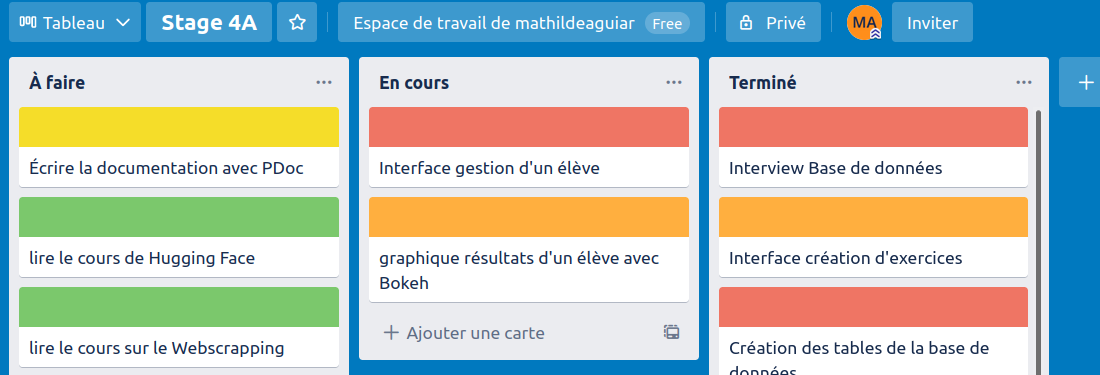
\includegraphics[scale=0.4]{trello.png}
    \caption{Une partie du Kanban de notre projet}
    \label{fig:trello}
\end{figure}

\subsubsection{Git}
Pour la gestion de mon code j'ai bien sûr utilisé Git (associé à GitHub et VisualStudio Code). Git m'a permis de pouvoir organiser mon développement  car même si j'étais seule je devais quand même garder mon code structuré. À chaque nouvel aspect de mon développement je créais une branche et à chaque nouvelle fonctionnalité terminée et validée je pouvais alors merge ma branche. Comme je travaillais seule, je n'ai pas eu à régler de conflit. 

\subsubsection{Adobe XD}
Pour réaliser les maquettes de mes interfaces j'ai utilisé AdobeXD, un logiciel de la suite Adobe. Ce logiciel nécessite un peu de prise en main et je n'ai pas découvert toutes les fonctionnalités disponibles du logiciel. Cependant mon utilisation assez basique m'a permis de réaliser facilement des maquettes simples. \textit{Voir certaines de mes maquettes aux annexes 10 et 11.}


\subsubsection{Visual Studio Code}
Pour la partie développement Web j'ai utilisé l'IDE  VisualStudio Code qui, avec les extensions Python, inclu un debugger Python. J'avais déjà l'habitude d'utiliser VS Code pendant l'année scolaire je n'ai donc pas eu à me réadapter à un nouvel IDE.

\subsubsection{Python Flask}

Pour réaliser notre exerciseur mon tuteur m’a suggéré d’utiliser le framework léger Python Flask. Celui-ci est particulièrement intéressant car il permet de générer des pages Web simplement et est extrêmement modulable grâce aux nombreux plugins que l’on peut lui adjoindre. Il permet tout de même de gérer les sessions, les routes et le serveur de développement. \\
Flask, couplé avec un système de base de données comme SQLAlchemy, se base sur le modèle MVT : Modèle, Vue, Template. La partie Modèle concerne tout ce qui va être intéractions avec la base de données, la partie Vue est là on l'on gère nos routes (les URLs des pages ainsi que ce qu'il faut transmettre aux templates), enfin les Templates sont les pages HTML qui affichent et structurent les variables passées via notre Vue. Le modèle MVT est plutôt intuitif et ressemble au MVC utilisé dans le projet Java du S6. 
Comme spécifié précédemment le Modèle est celui qui contient le code de notre base de données et les méthodes associées à celle-ci. Dans mon projet j'ai utilisé l'ORM (Object Relational Mapping) SQLAlchemy qui me permet d'écrire mes requêtes et de définir mes tables de base de données directement avec des objets Python tout en me basant sur une base de données utilisant les mécanismes de SQLite. L'avantage d'utiliser des objets plutôt que des Strings directement est que cela ne permet pas de faire des attaques à l'injection SQL. \textit{Voir figure 3.}

\begin{figure}[h]
    \centering
    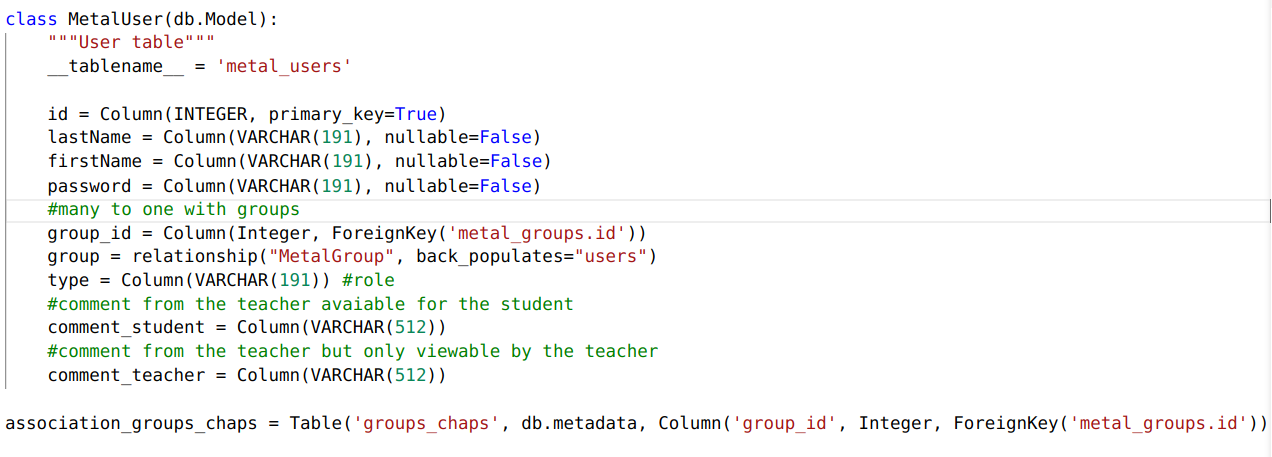
\includegraphics[scale=0.3]{ex_models.png}
    \caption{Extrait de notre modèle - Table "Utilisateur" }
    \label{fig:ex_models}
\end{figure}

La Vue est là où sont définies nos routes, nos URLs. C'est la Vue qui fait le lien entre la base de données et les templates. Elles exécutent les requêtes définies dans le Modèle et passent leurs résultats aux templates. Elle fait aussi le lien entre les autres classes (comme celles définies pour les formulaires) et les templates correspondantes. \textit{Voir figure 4.}

\begin{figure}[h]
    \centering
    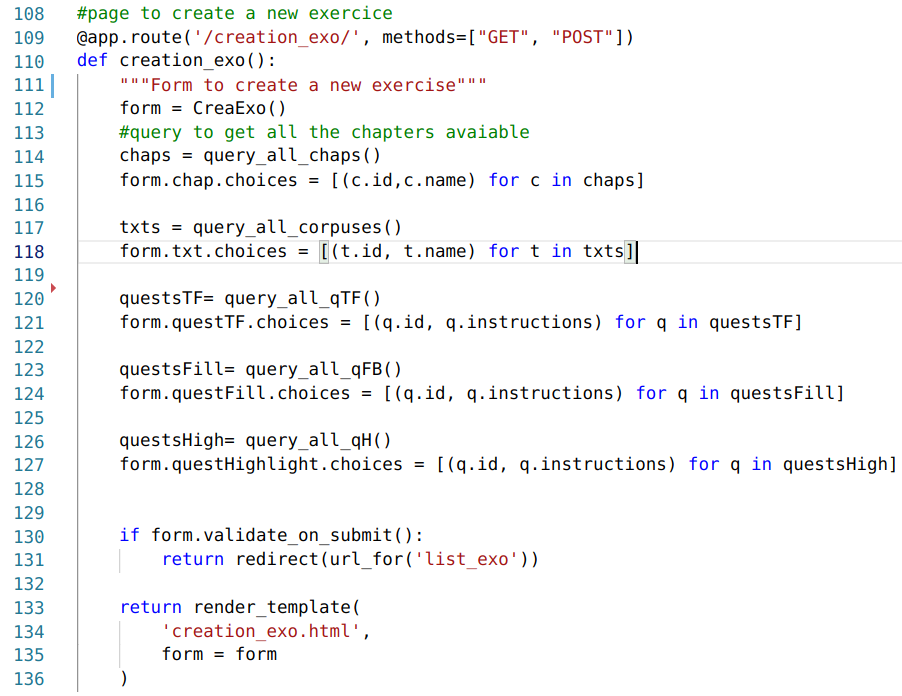
\includegraphics[scale=0.3]{ex_views.png}
    \caption{Extrait de la Vue}
    \label{fig:ex_views}
\end{figure}

Ici nous avons tout d'abord la définition de l'URL via \textbf{$@$app.route()} (ligne 109). Puis l'instanciation du formulaire de création d'exercices (ligne 112 à 127). De la ligne 130 à 131 on a une redirection vers la template 'liste d'exercices' si l'utilisateur soumet le formulaire rempli et que celui-ci est valide. Enfin le \textbf{render\_template()} permet de savoir quelle template représenter et de transmettre la variable "form" à la template.   \\
En ce qui concerne tous les formulaires de saisie, j'ai utilisé \textbf{Flask WTForms} ce qui m'a permis de facilement définir  les champs voulus. \textit{Voir figure 5.}



\begin{figure}[h]
    \centering
    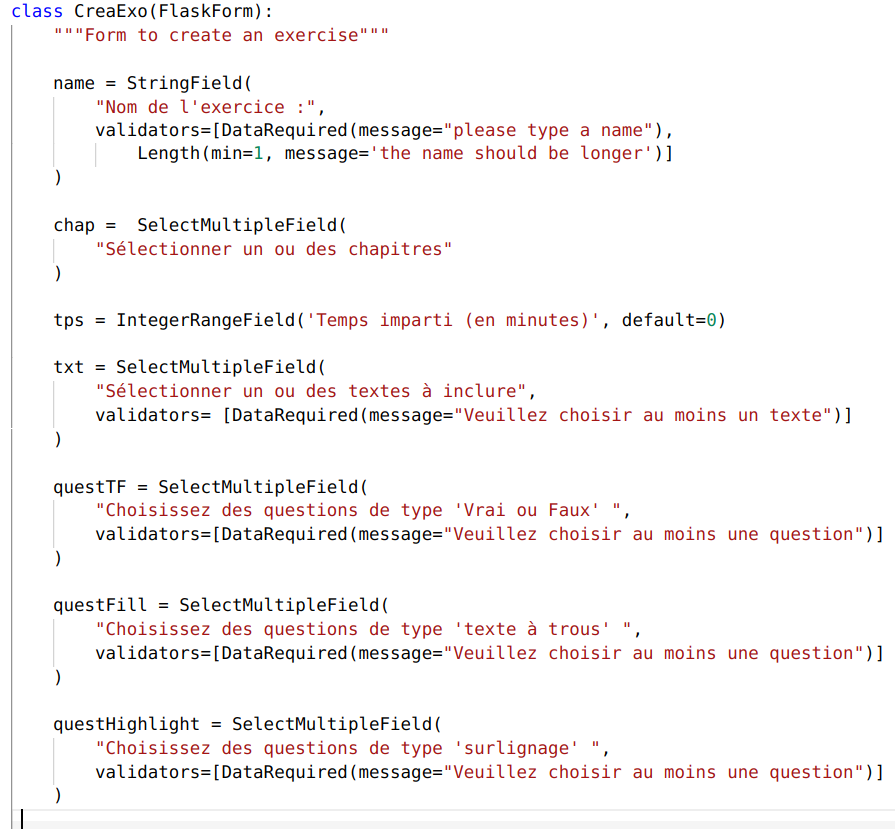
\includegraphics[scale=0.3]{ex_wtforms.png}
    \caption{Exemple de formulaire WTForms - formulaire de création d'exercices}
    \label{fig:ex_wtforms}
\end{figure}

\clearpage

Les templates quand à elles sont des pages HTML qui représentent ce que la Vue leur transmet. Elles sont très pratiques car il y a un système d'héritage ce qui permet de ne pas répéter plusieurs morceaux de code identiques. On peut définir les blocs de code à inclure dans une autre template via \textbf{ \{\% block content \%\} \{\%endblock\%\}} et inclure un bloc de code via \textbf{ \{\% include 'file.html' \%\} }. \textit{Voir figure 6}. 

\begin{figure}[h]
    \centering
    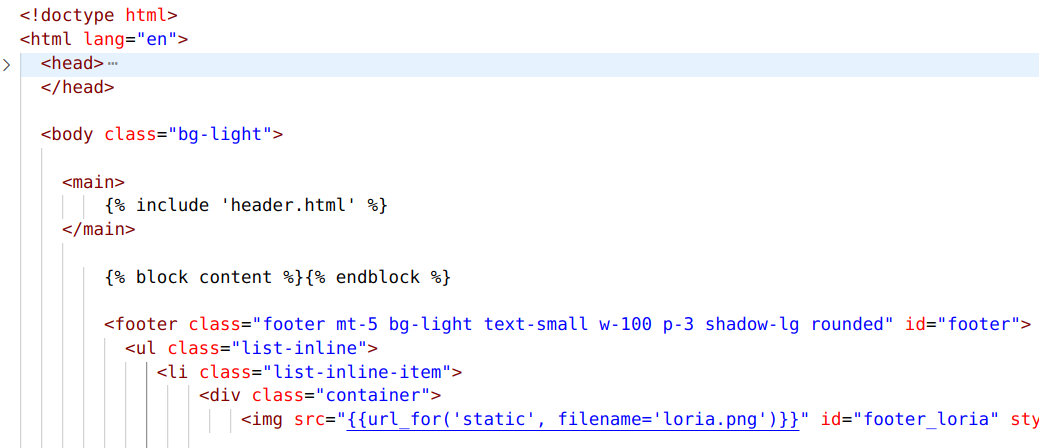
\includegraphics[scale=0.3]{ex_block_base.png}
    \caption{Un extrait d'une template - base.html}
    \label{fig:ex_temp}
\end{figure}

Moins lourde que la version PHP précédente, Flask a donc été retenu pour le développement de notre application.

\subsubsection{Google Collabs}
Pour ma partie "recherche" j'ai utilisé les notebooks disponibles sur Google Collabs. Ils sont largement utilisés dans la communauté Natural Language Processing (NLP) et c'est d'ailleurs ce que l'on avait utilisé pour les TP de Communication Langagière. L'avantage de Collabs c'est qu'ils allient à la fois un notebook et un environnement d'exécution GPU (je n'ai pas de GPU sur ma machine), ce qui permet d'accélérer les exécutions. 
De plus, le concept de notebook est très pratique pour des travaux de type "recherche". Il me permet de noter au fur et à mesure mes observations, les ressources utilisées et des commentaires bien plus fournis que de simple commentaires Python. En utilisant les notebooks on peut structurer notre démarche expérimentale directement avec des extraits de code. 

\subsubsection{Hugging Face}
Hugging Face est une organisation/entreprise spécialisée dans le Traitement Automatique des Langues. Elle fourni de nombreux modèles pré-entraînés, tokenizers, datasets et autres outils pour réaliser les tâches les plus communes de NLP. L'avantage de Hugging Face est qu'ils mettent à disposition à la fois une solution payante mais que leurs modèles pré-entraînés sont disponibles gratuitement et que l'on peut les utiliser librement. C'est une solution très pratique car, en ayant des modèles \textbf{pré-entraînés}, cela me permet de ne pas à réaliser l'entraînement de 0 qui est à la fois coûteuse en temps mais aussi en énergie. Je ne réaliserais qu'un entraînement "rapide", le \textbf{fine-tuning}, qui visera à entraîner mon modèle sur des données ciblées pour qu'il réponde plus particulièrement à la tâche que je souhaite réaliser. 

\subsection{Organisation du travail}

J’ai travaillé en grande partie en autonomie et j’ai donc eu une liberté quasi totale sur ma façon d’organiser mon travail. M.Parmentier et moi avions des réunions hebdomadaires au laboratoire pour faire un point sur mon avancement et définir les objectifs de la semaine à venir. Durant ses réunions nous échangions également sur la façon dont nous imaginions notre exerciseur. 


\begin{figure}[h]
    \centering
    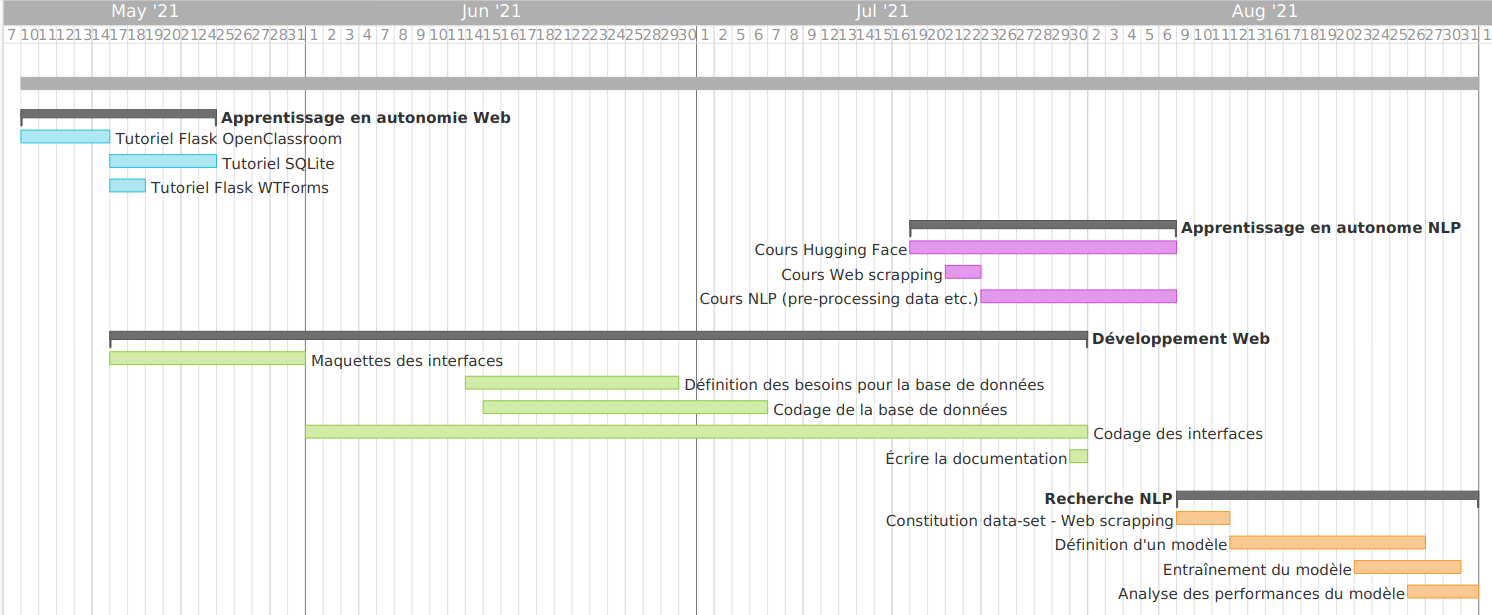
\includegraphics[scale=0.35]{gantt.png}
    \caption{Diagramme de Gantt de mon stage}
    \label{fig:gantt}
\end{figure}

Globalement mon stage s'est déroulé comme suit :
\begin{itemize}
    \item 1ère semaine : première utilisation de Flask. Réalisation du tutoriel OpenClassrooms. 
    
    \item 2ème - 3ème semaine : Prise en main de SQLite et WTForms avec la réalisation d'une interface de gestion d'un magasin de disques/CD. Découverte des interfaces précédemment réalisées par l'ingénieur précédent. Conception de maquettes des futures interfaces.
    
    \item 4ème semaine : Début de la bifurcation vers notre projet final. À partir de la base de données du tutoriel SQLite, je "mappe" des classes/tables qui pourrait être des classes de notre application finale. Je commence à coder les interfaces et formulaires de création d'exercices.
    
    \item 5ème semaine : Réel début du développement du projet. Les semaines précédentes m'ont permises d'acquérir des bonnes bases en Flask et en SQLite/SQLAlchemy ce qui facilite largement la mise en place du projet. J'ai commencé par coder le formulaire de création d'exercices, la page d'accueil avec une recherche générale dans toute la base ainsi que la page de "validation" des notions trouvées grâce à notre analyseur. Réalisation de la 1ère version de la base de données, directement inspirée par celle produite par l'ingénieur précédent.
    
    \item 6ème-14ème semaine : Je continue sur ma lancée en développant les interfaces de création de chapitres, de sessions d'exercices, etc. M.Parmentier et moi discutons d'une nouvelle configuration de la base de données. Je réalise une nouvelle structure de la base de données en réalisant un graphe UML. En suite je code cette dernière. Je finalise mes interfaces. J'écris la documentation.
    
    \item 15ème semaine : Basculement vers la partie NLP. Je lis les cours sur le Web scrapping, les cours de Hugging Face pour utiliser leurs modèles. Je commence à tester les techniques de Webscrapping vues dans les cours. Je peaufine les derniers détails de mes interfaces Web.
    
    \item 16ème semaine : Je m'occupe de la réalisation de mon dataset, j'explore les données récoltées et je vérifient qu'elles soient exploitables et cohérentes. Je commence à explorer une façon de réaliser un modèle performant.
    
    \item 17ème semaine - fin de mon stage : J'ajuste mon modèle. J'analyse les résultats obtenus. 

\end{itemize}

Nous avons préféré mettre l'accent sur la partie développement Web. En effet cette partie était celle où je pouvais le plus facilement obtenir des résultats concrets et intégrables dans notre application finale. La seconde partie de mon stage étant plus expérimentale, je ne suis pas certaine d'obtenir des bons résultats et même arriver au bout de mes expérimentations.  

\subsection{Missions réalisées}

\subsubsection{Développement Web}

Tout d’abord j’ai passé les premières semaines de mon stage à découvrir Flask ainsi que quelqu’un de ses plugins. J’ai réalisé différents tutoriels et bien étudié la documentation de chaque plugin au fur et à mesure de mon développement. Le 1er tutoriel que j’ai réalisé fut un simple site (voir annexe figure 12). Ce tutoriel m’a permis de découvrir les bases de Flask, le MVT (Modèle, Vue, Template) avec l’utilisation de templates Jinja, mais aussi de découvrir un ORM (Object–relational mapping) avec l’utilisation de SQLAlchemy. \\

J’ai ensuite fait un tutoriel pour découvrir SQLite. Ainsi qu’un autre, rapide, pour découvrir la génération de formulaires avec le plugin Flask WTForms. Pour m’entraîner à maîtriser ses 2 concepts j’ai réalisé une interface de gestion de base de données d’un magasin de disques musicaux. Je n’ai pas utilisé d’ORM cette fois-ci et j’ai simplement écrit mes requêtes SQL via des simples Strings. \textit{Voir figure 13 en annexe}. \\

En parallèle de la réalisation de ses tutoriels, j’ai réalisé des maquettes des interfaces de notre application à l’aide de Adobe XD. Cette étape était pour moi nécessaire car j’avais besoin d’une représentation visuelle de ce à quoi notre application pourrait ressembler. De plus cela nous a permis à M.Parmentier et moi d’échanger plus facilement sur les fonctionnalités que notre application devrait posséder.   \textit{Voir figures 14 et 16 en annexe}. \\
 
Enfin une fois après avoir maîtrisé tous ses nouveaux frameworks j’ai pu me lancer dans la réalisation des interfaces de l’exerciseur destinées à l’enseignant. \\

Tout d’abord j’ai commencé par reprendre la base de données créée par le précédent ingénieur. Cette dernière comportait 41 tables, ce qui nous paraissait excessif, et certaines fonctionnalités n'étaient plus intéressantes. Pour me guider dans la redéfinition de la base de données je me suis inspirée du partiel de base de données du semestre 7. J’ai commencé par faire une "interview client" en définissant toutes les fonctionnalités et les choses réalisables avec nos interfaces. Malheureusement je n’ai pas pu faire l’interview d’un enseignant j’ai donc imaginé un dialogue par moi-même. De plus mes nombreux échanges avec M.Parmentier m’ont permis de mieux définir les tenants et aboutissants de notre projet. J’ai ensuite réalisé un graphe UML \textit{(voir en annexe les figures 18 et 19)}. Enfin à partir de celui-ci j’ai pu coder la base de données avec l’ORM SQLAlchemy, celle-ci utilisant le dialecte SQLite. \\

En parallèle de la définition de la base de données, j’ai développé les interfaces "enseignant" (\textit{voir figure 20 en annexe}). Pour ce faire, je me suis appuyée sur les maquettes réalisées avec Adobe XD. J’ai utilisé les connaissances acquises avec les tutoriels réalisés pendant les premières semaines pour mettre en place les différentes interfaces. J’ai donc utilisé dans la mesure du possible les macros de Bootstrap Flask et complété certains aspects avec Bootstrap seul. 
Notre projet a la structure suivante (\textit{voir figure 8}):
\begin{itemize}
    \item Les fichiers 'config.py' et 'run.py' servent à lancer l'exécution en respectant des hyper paramètres de configuration.
    
    \item Le dossier 'app' est là où se trouve toute notre application
    
    \item Il comporte un dossier 'static' qui contient tous les fichiers dit statiques : images, .css .js, etc.
    
    \item  Un dossier 'templates' qui contient toutes nos templates (fichiers HTML)
    
    \item 'views.py' qui est notre Vue comprenant les routes
    
    \item 'Models.py' qui comprend la définition de la base de données ainsi que toutes les fonctions pour réaliser des requêtes
    
    \item D'autres fichiers .py comme par exemple 'creation\_session.py' qui sont des formulaires Flask WTForms.

\end{itemize}

\begin{figure}[h]
    \centering
    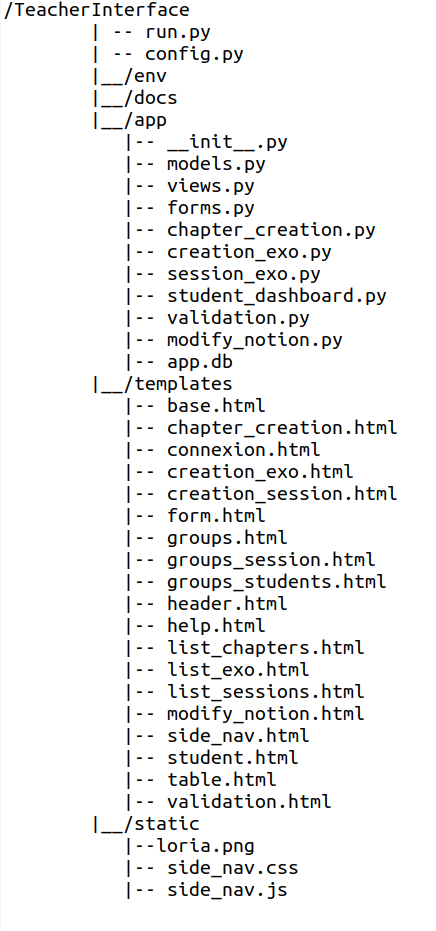
\includegraphics[scale=0.4]{structure_Flask.png}
    \caption{Structure des fichiers des interfaces}
    \label{fig:structure_flask}
\end{figure}


En ce qui concerne toutes les interfaces de création d’exercices, de sessions d’exercices ou de chapitres j’ai utilisé des formulaires basés sur Flask WTForms. Ce plugin rend la création de formulaires vraiment très simple. J'ai utilisé un module complémentaire, Flask CKEditor, pour offrir la possibilité d'ajouter du rich text (texte gras, italique, surlignage, snippets de code, etc.) dans la saisie de champ du formulaire. \textit{Voir figure 17 en annexe.} \\ 


Pour l'affichage de graphiques, notamment dans l'interface de gestion des résultats d'un élève, j'ai utilisé Bokeh. Il m'a permis de créer des graphiques intéractifs des notes obtenues par un élèves et tout cela directement inclu dans mes templates Jinja. \\

Pour finir, j'ai utilisé Pdoc pour créer une documentation de mon code. Mes fichiers .py sont plutôt longs et comportent de nombreuses fonctions (models.py avec environ 1000 lignes par exemple). Grâce à Pdoc j'ai non seulement pu générer une documentation au format HTML (qui d'ailleurs utilise Jinja 2 aussi) mais aussi une documentation consultable dans l'IDE (comme la JavaDoc dans Eclipse).


\subsubsection{Partie "recherche" sur le traitement du langage naturel}
\textbf{Définition du sujet :} \\
Pour cette partie, M. Parmentier n'avait pas d'exigence particulière dans le sens où il s'agissait d'un travail exploratoire. Je travaille d'ailleurs encore sur cette partie au moment où je rédige ce rapport. \\
Tout d'abord il a fallu définir notre problématique et les résultats souhaités de la part de notre modèle. Nous avons décidé de créer un modèle qui serait capable de labéliser des textes et d'en extraire les sujets principaux. \\

Pour cela je me suis organisée comme ceci-ci : \\
J'ai d'abord dû rassembler des ressources pertinentes pour mon auto-formation. Je me suis appuyée sur des cours dispensés par M.Parmentier et certaines de ses collègues dans le cadre du Master TAL. J'ai également décidé d'utiliser les Transformers (librairies) développées par Hugging Face, j'ai donc suivi les cours créés par les développeurs de Hugging Face. J'ai également revu les cours et TP réalisés en cours de Communication Langagière au S8. \\


\begin{figure}[h]
    \centering
    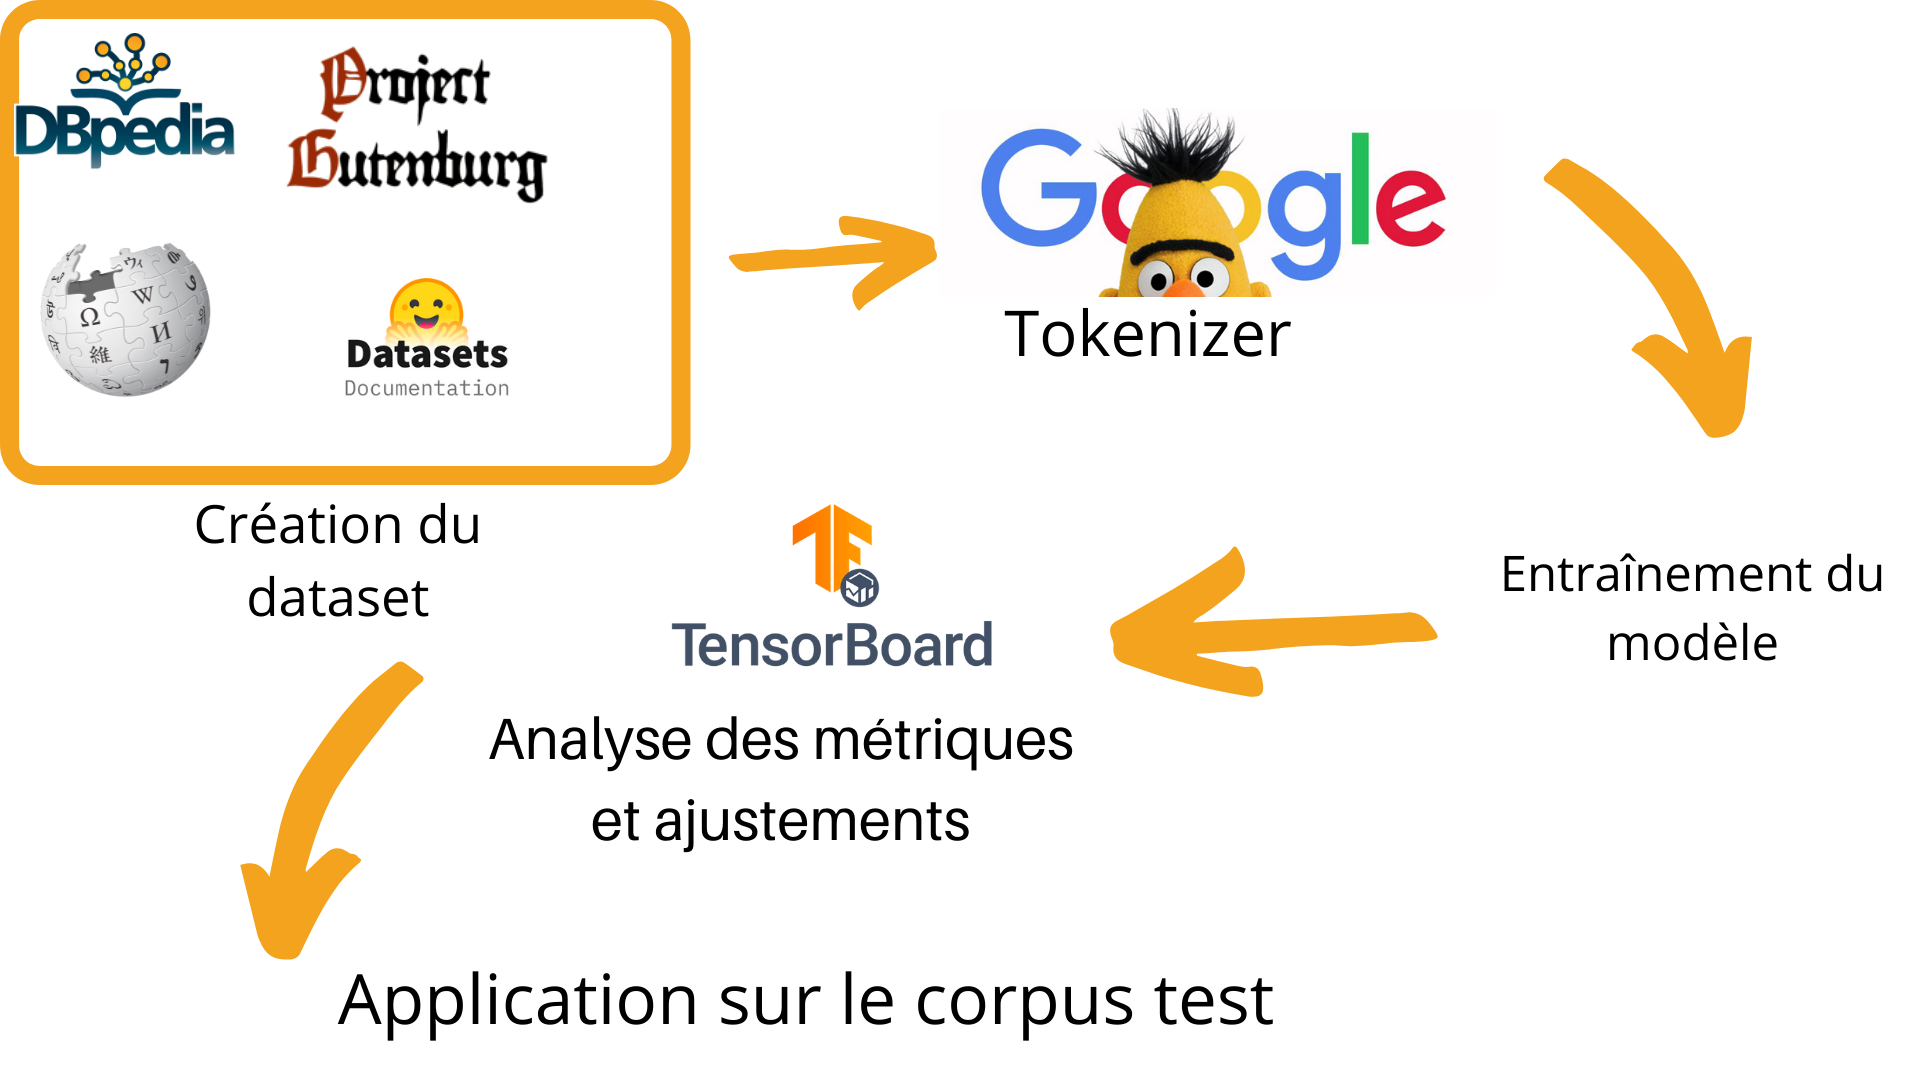
\includegraphics[scale=0.3]{graphe NLP.png}
    \caption{Cycle de développement de mon modèle}
    \label{fig:NLP}
\end{figure}


\textbf{Collecte des données d'entraînement et de test} \\
Une fois après avoir acquis quelques connaissances j'ai commencé par réaliser mon jeu de données. Cette partie était toute nouvelle pour moi car nous n'avons jamais abordé cet aspect en cours de communication langagière (les data-sets nous étaient toujours fournis). J'ai donc réalisé du Webscraping sur les ressources disponibles sur le site Gutenberg. J'ai donc récolté une collection de ebooks classiques en français.
J'ai également réalisé des requêtes sur la collection de données WikiData et Dbpedia grâce au wrapper Python SPARQL (pour Dbpedia) et au wrapper WPTools (pour Wikipedia). \\
En effet Dbpedia et Wikipedia sont des encyclopédies libres qui mettent à disposition les ressources entrées par les utilisateurs. Elles sont structurées selon le modèle RDF. C'est à dire que les ressources présentes sur ses sites sont organisées de façon structurée. Par exemple, chaque page Dbpedia est composée d'un \textbf{title}, d'un \textbf{label}, etc. Cette structure va nous permettre de réaliser des requêtes très facilement et de n'extraire que le contenu dont nous avons besoin. \\

\clearpage

\textbf{Choix du tokenizer} \\
Une fois les données récoltées j'ai du les traiter et les rendre exploitables par notre modèle. J'ai donc commencé par tester plusieurs méthodes de \textit{pre-processing}. Cette étape consiste en la conversion d'un token en un entier compréhensible par le modèle. Pour la tâche de topic modeling j'avais besoin d'avoir un  tokenizer réunissant les propriétés suivantes :

\begin{itemize}
    \item Suppression de la ponctuation 
    \item Passage en minuscules de certains tokens 
    \item Suppression des mots fréquents (et qui comportent donc peu d'information)
\end{itemize} 


La question s'est posée de savoir si je devais réaliser un tokenizer de "A à Z" ou plutôt utiliser un tokenizer déjà préexistant. J'ai donc d'abord réaliser mon propre tokenizer avec la bibliothèque NLTK. J'ai réalisé quelques tests sur des phrases en français et des tests sur des phrases en japonais. J'obtiens de bons résultats sur les collections de phrases françaises mais il ne fonctionne pas sur les collection de phrases japonaises. Même si pour l'instant mon modèle ne verra que des phrases françaises, j'ai préféré laisser ce tokenizer de côté. 
J'ai donc décidé de me tourner vers des Tokenizers plus puissants et déjà pré-entraînés. J'ai décidé d'utiliser des Tokenizers mis à disposition par Hugging Face. En partant sur tokenizer pré-entrainé il faut que celui-ci corresponde au modèle utilisé, je suis donc passée à l'étape "choix du modèle". \\

\textbf{Choix et définition du modèle} \\
Notre tâche à réaliser est du \textit{topic modeling}, pour se faire il faut utiliser un modèle à encodeur unique. 
Parmi les modèles disponibles sur le \textbf{\href{https://huggingface.co/models}{'Hub' de Hugging Face }}, j'ai décidé de faire des essais avec les modèles BERT, développé par Google, et DistillBERT, développé par Hugging Face. Ces 2 modèles sont bien adaptés pour la tâche de topic modeling. L'avantage de DistillBERT par rapport à BERT est sa rapidité et sa légèreté tout en gardant des résultats proche de ceux de BERT (seulement 0.6 \% de moins d'\textit{accuracy} sur les mêmes jeux de tests, \textit{voir figure 11, table 2}). \\

\clearpage

\begin{figure}[h]
    \centering
    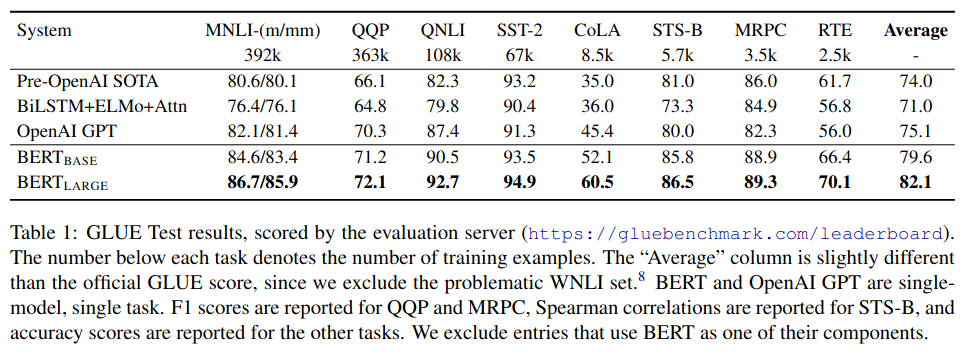
\includegraphics[scale=0.45]{bench_BERT.png}
    \caption{BERT benchmarks}
    \label{fig:bench_bert}
\end{figure}


\begin{figure}[h]
    \centering
    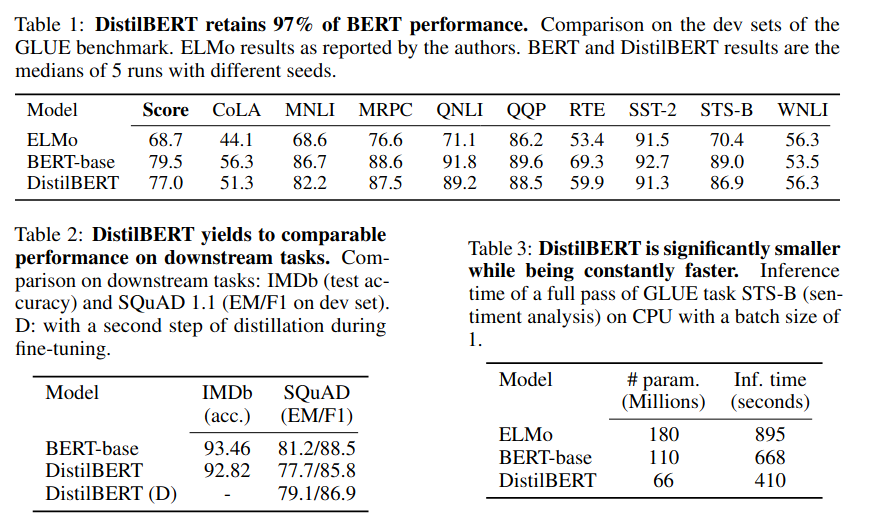
\includegraphics[scale=0.45]{bench_distillBERT.png}
    \caption{DistillBERT benchmarks}
    \label{fig:bench_distill}
\end{figure}

 \clearpage

\textbf{Entraînement et analyse des résultats} \\
\textit{Attention ! Cette partie de mon stage est toujours en cours !}

Une fois choisi, il est temps de passer à l'entraînement du modèle. Je possède donc un jeu de données d'entraînement et c'est à partir de celles-ci que je vais pouvoir \textit{fine-tune} mon modèle. Je vais donc devoir trouver les bons paramètres à utiliser pour obtenir une \textit{accuracy} (probabilité que la réponse donnée par le modèle soit juste) élevée mais aussi pour avoir un temps d'exécution pas trop long. \\ 

\textbf{Tests} \\
Une fois mon modèle satisfaisant je vais pouvoir passer mon jeu de données test au modèle. Je vais m'assurer que les résultats obtenus sont ceux attendus et je vais ajuster encore une fois mes paramètres pour voir si je peux obtenir de meilleurs résultats.  


\subsection{Difficultés rencontrées}

Dans l’ensemble, la réalisation des interfaces de l’exerciseur s’est plutôt bien passée. Même si j’ai rencontré quelques embûches, le temps passé sur une difficulté n’a jamais été très long. De plus, le fait d’avoir plusieurs tâches à faire en parallèle m’a permis de ne pas "rester bloquée" sur la tâche qui me donnait du fil à retordre. \\

Une des difficultés majeures fut la réalisation de la base de données. Le modèle conçu précédemment ne convenait plus tout à fait à l'idée que nous nous faisions de l’exerciseur. En effet, l'ingénieur précédent avait imaginé certaines fonctionnalités comme la \textit{gamification} (l'apprentissage par le jeu) des exercices, la possibilité d'obtenir des récompenses au nombre d'exercices réalisés, etc. Certaines interfaces étaient un petit peu désuètes et il fallait un peu les restructurer.   
De plus, le fichier contenant la base de données n’était pas commenté/documenté, il fallait donc interpréter soi-même certains champs définis par l’ingénieur précédent.  De plus, sans "client" avec lequel discuter il est plus compliqué de définir les besoins des élèves et enseignants qui vont utiliser la plateforme. \\

Une interface a été plus compliquée à imaginer et à coder que les autres, l'interface de l'analyse d'un texte par l'analyseur. En effet je me suis inspirée de l'interface réalisée par l'ingénieur précédent mais j'ai souhaité remodeler quelques aspects. Cette interface nécessite de garder une base de code commune mais possède de nombreuses fonctionnalités et doit donc être très modulable. J'ai donc dû jouer sur l'utilisation de différents paramètres dans les routes. Mais la difficulté principale reste le fait de ne pas pouvoir tester avec de vraies données ce que l'analyseur nous renvoie. Je pense que l'implémentation que j'ai réalisée sera sujette à encore nombreux changements quand l'analyseur sera stabilisé. 

\subsection{Améliorations possibles}
À l’heure où j’écris ce rapport, mon stage n’est pas encore terminé. Je peux donc encore continuer à améliorer mon travail. Cependant je vois quelques points que je n’aurais pas le temps d’aborder. \\

\textbf{L’internationalisation :} Dans la version actuelle, notre exerciseur est uniquement en français. J’ai voulu réaliser une version anglaise de l’interface à l’aide de Babel Flask. Ce plugin Flask permet, à partir de Strings balisée, de générer un fichier .po qui sert de dictionnaire pour les termes à traduire. Cependant je me suis rendue compte que ce plugin ne me serait pas d’une grande aide. En effet les phrases balisées doivent être des Strings "brutes" et non contenues dans une variable. Il faudrait donc un autre plugin ou une autre solution pour traduire nos interfaces mais que celles-ci restent également facile à maintenir. \\

\textbf{L'analyse des textes :}  Compte tenu de la date de rendu de ce rapport, je n'ai pas fini de travailler sur la partie NLP. De plus, cette partie est plus compliquée à appréhender pour moi et nous ne sommes pas sûrs d'obtenir des résultats satisfaisants à la date de fin de mon stage. \\

\textbf{Avoir un retour "utilisateur" :} L'application disponible actuellement n'a pas vraiment été testée par un enseignant (et encore moins par un élève). Au cours de mon développement j'ai utilisé des valeurs factices pour remplir ma base de données et avoir une idée de ce à quoi mon interface va ressembler. Cependant je n'ai pas eu de vrai retours sur l'ergonomie de mon interface ainsi que sa facilité d'utilisation. 
Un autre point intéressant à aborder serait que notre interface soit utilisable par le plus grand nombre, par conséquent qu'elle comporte des modules \textit{d'accessibilité} (pour les malvoyants par exemple). 


\section{Bilan personnel}


Ce stage m’a permis de parfaire mes compétences en Python et découvrir Flask. Je ne savais pas qu’il était possible de coder des pages Web à l’aide de Python. Naturellement j’ai aussi pu développer mes compétences en HTML/CSS et pu approfondir mon utilisation de Bootstrap. \\
J'ai également pu étendre mes connaissances en traitement du langage naturel. J'ai approfondi ce que l'on avait vu en TP de Communication Langagière et je l'ai réutilisé pour un cas concret. Je connais maintenant les étapes à réaliser pour produire un modèle de Topic Modeling et les problématiques que je pourrais rencontrer en réalisant ce type de projet. \\
De plus, j'ai pu développer mes capacités d'apprentissage en autonomie. En effet, je n'avais jamais utilisé Flask et les autres technologies citées plus haut et j'ai beaucoup apprécié le fait de les apprendre par moi-même et de me les approprier. J'ai trouvé ma propre méthode d'apprentissage et mon propre rythme de travail. \\
J’ai pu également mettre en œuvre les notions apprises en cours de base de données, via la définition et la mise en place de la base de données, ainsi que la réalisation de graphes UML. \\
J'ai parfait mes compétences en développement logiciel. J'ai pu mettre en pratique l'utilisation de Git. \\
De plus, cette expérience m’a permis de découvrir les conditions de travail dans un laboratoire de recherche. J’ai particulièrement apprécié la liberté d’organisation et de répartition de la charge de travail que m’a offert ce stage. \\

Je remercie également M.Parmentier de m'avoir fait découvrir de  nombreuses ressources autour des langues et du Traitement des Langues. Ce stage ne fait que me conforter dans l'envie de continuer dans cette voie. 

\subsection{Compétences développées}

\subsubsection*{Capacité à mettre en place des dispositifs expérimentaux  }

Pour la partie "recherche" de mon stage j'ai dû mettre en place un dispositif expérimental. Pour mener à bien ma mission je me suis organisée selon les étapes suivantes. \\
Tout d'abord moi et mon tuteur avons commencé par définir l'objectif de notre modèle et les résultats attendus par celui-ci. \\
Ensuite j'ai recherché des ressources pour pouvoir m'auto-former et comprendre mon sujet. \\
Une fois avoir lu et compris ses ressources j'ai pu savoir quelles étapes je devais réaliser. \\
Avant de me lancer dans le projet final j'ai exploré les 2 grosses librairies que j'allais utiliser. J'ai écrit des petites requêtes en SPARQL et j'ai récupéré des contenus de pages Wikipedia. J'ai également  écrit des petits tests simples pour tester les différents modèles de Hugging Face et voir ceux qui seront adaptés pour réaliser notre tâche. J'ai utilisé les \textbf{pipelines()} de Hugging Face pour voir comment leur modèles peuvent résoudre les tâches courantes de NLP. \\
Une fois à l'aise j'ai enfin pu passer au modèle final. J'ai donc procédé par étapes :

\begin{itemize}
    \item Constitution du dataset : web scrapping sur WikiData et Gutenberg
    
    \item Vérifier que les données traitées sont cohérentes et qu'elles correspondent à notre tâche
    
    \item Tokenization : j'utilise le tokenizer de Hugging Face pour que nos données soient exploitables par notre modèle. 
    
    \item Mise en batch (groupe de données) pour les étapes d'entraînement, de validation et de test.
    
    \item Définition des paramètres d'entraînement. 
    
    \item Entraînement du modèle (fine-tuning).
    
    \item Phase de test, où l'on donne au modèle des données jamais rencontrées.
    
    \item Analyse des résultats obtenus. 
    
\end{itemize}

Une fois nos tests réalisés une première fois on regarde les résultats obtenus par le modèle. Le premier essai n'étant pas satisfaisant on fait varier les paramètres de notre modèle. On peut aussi modifier le jeu de données utilisé pour le fine-tuning de notre modèle. 


\newpage

\section{Annexes}

\begin{figure}[h]
        \centering
        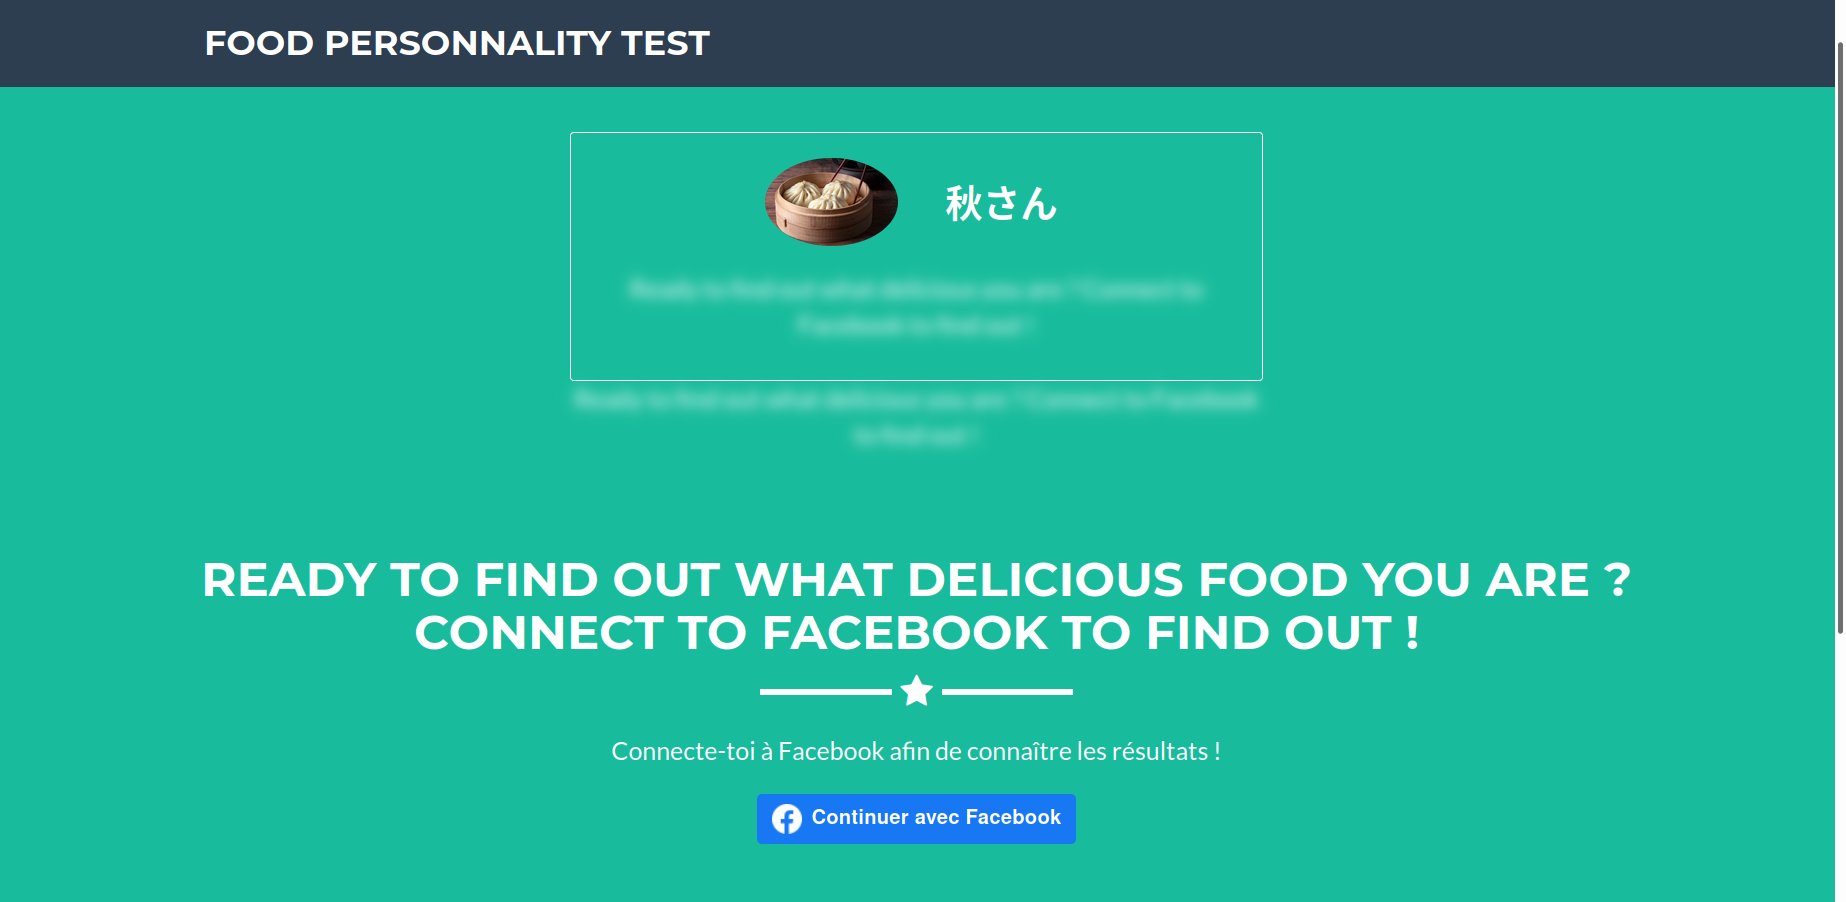
\includegraphics[scale=0.27]{tuto_OC.png}
        \caption{Tutoriel Flask OpenClassrooms}
        \label{fig:tuto_OC}
\end{figure}

\begin{figure}
    \centering
    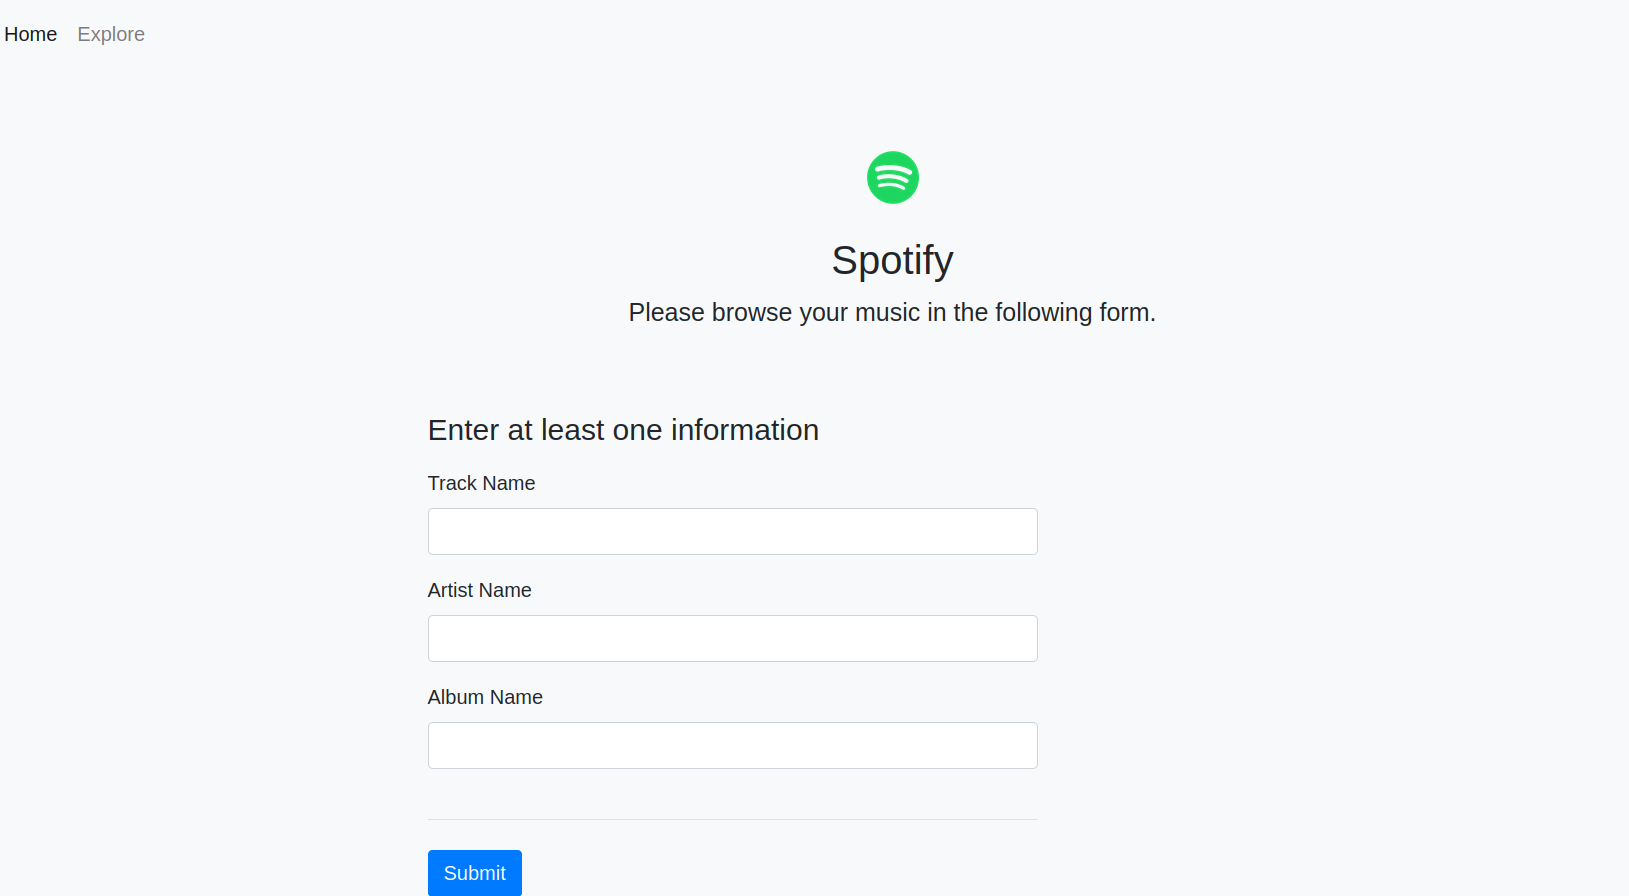
\includegraphics[scale=0.3]{tuto_sqlite.png}
    \caption{Tutoriel SQLite}
    \label{fig:tuto_sqlite}
\end{figure}

\begin{figure}
    \begin{subfigure}
        \centering
        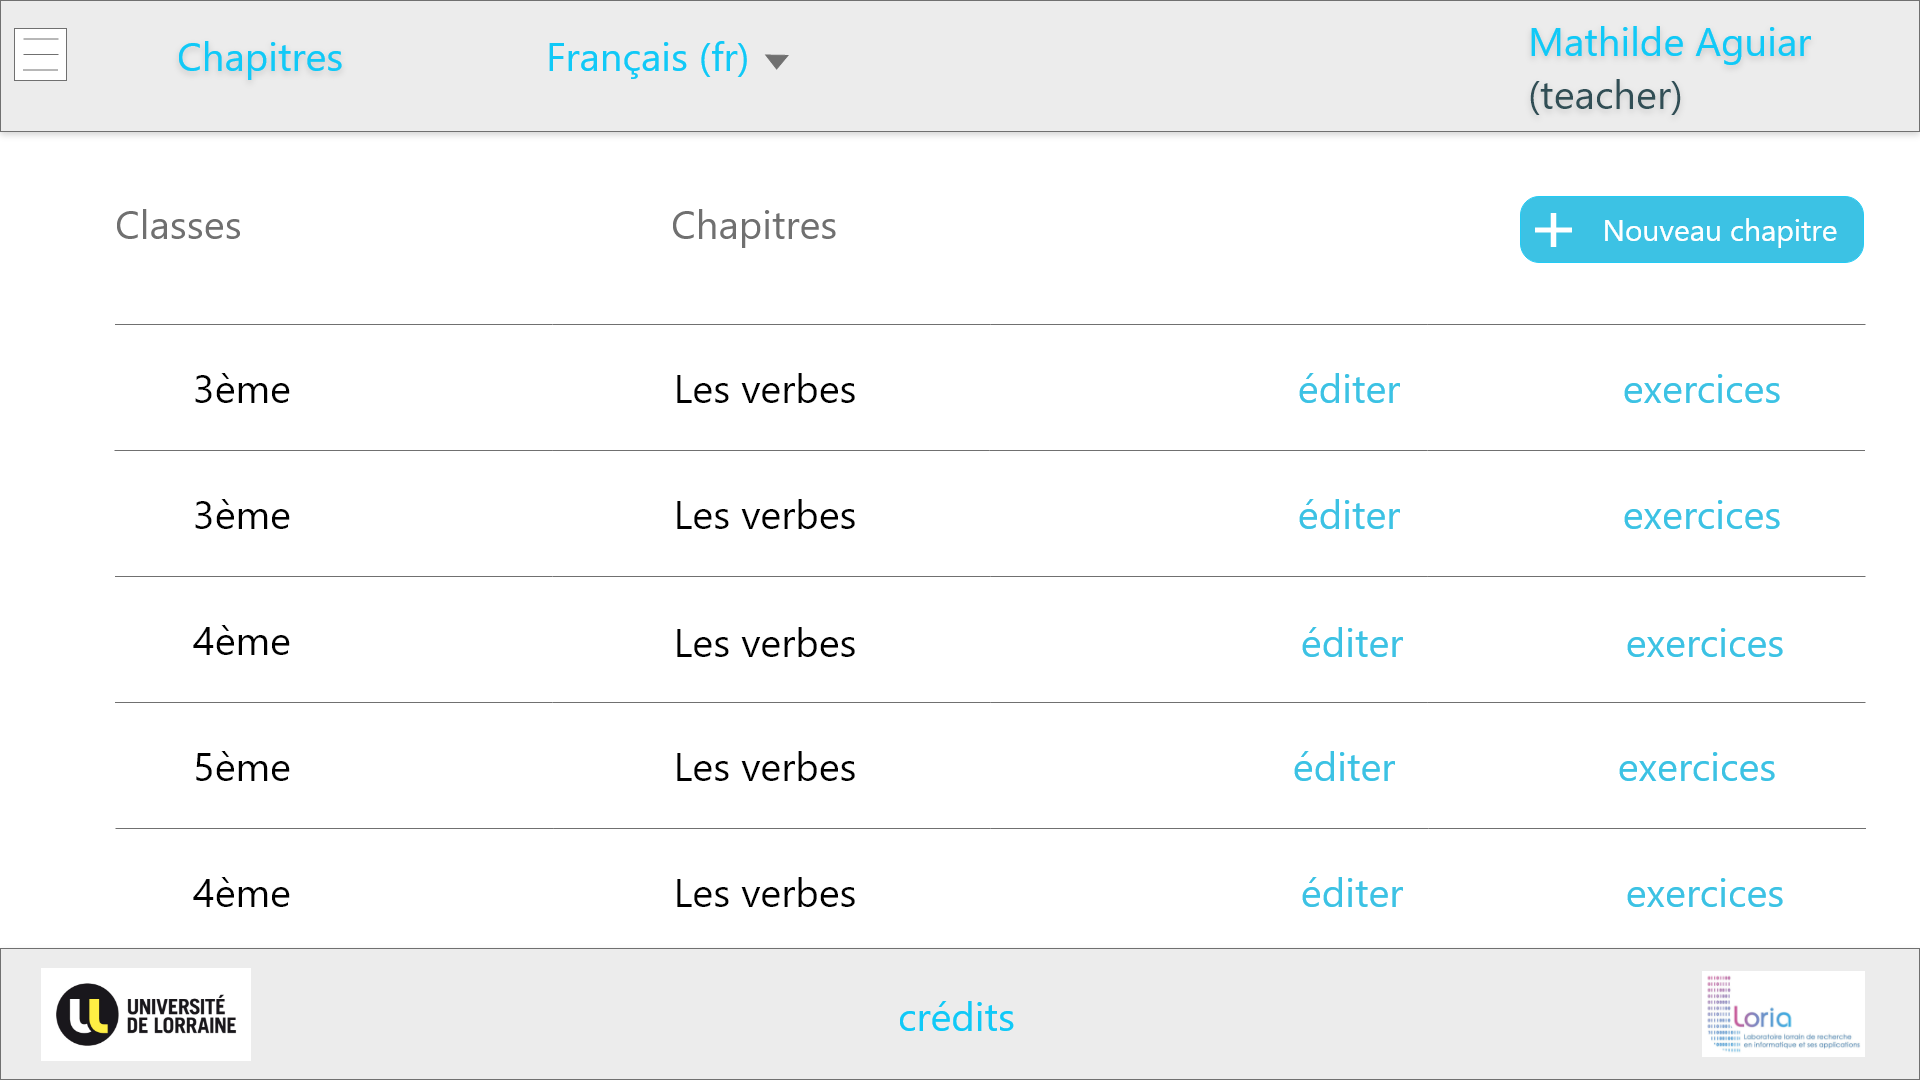
\includegraphics[scale=0.27]{Chapitres.png}
        \caption{Maquette de la liste des chapitres disponibles}
        \label{fig:maquette1}
    \end{subfigure}
    
    \begin{subfigure}
         \centering
        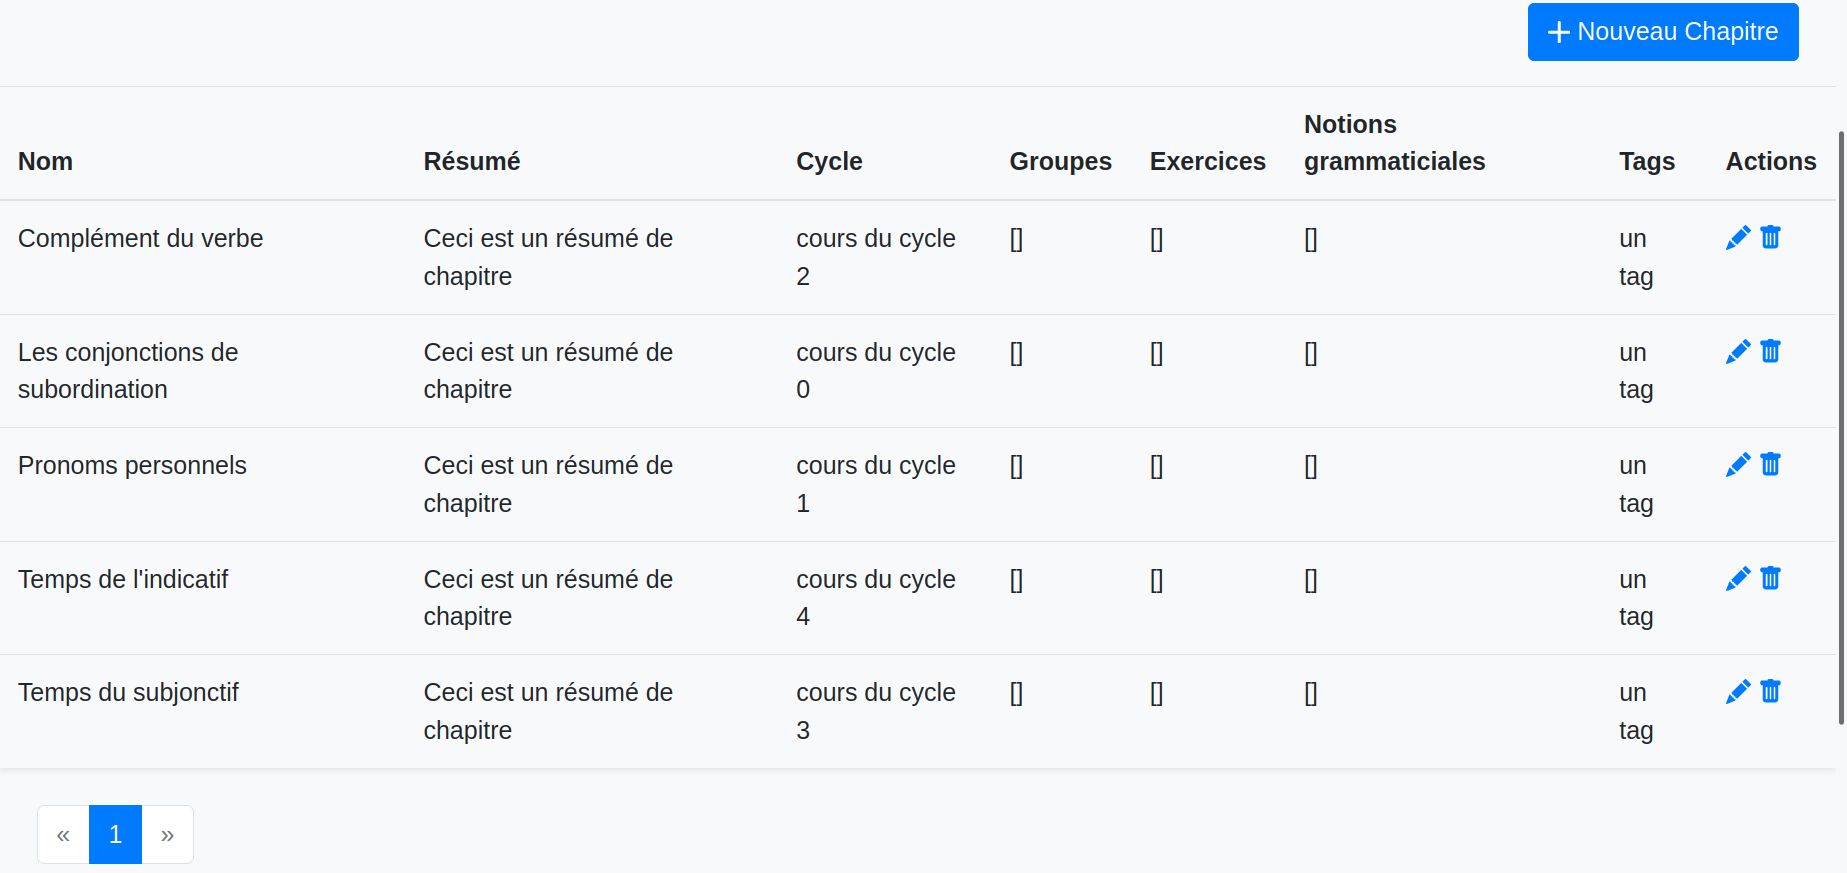
\includegraphics[scale=0.28]{table_chap.png}
        \caption{Interface des chapitres disponibles}
        \label{fig:table_chap}
    \end{subfigure}
    
    
\end{figure}



\begin{figure}
        \centering
        \includegraphics[scale=0.27]{chapitre - création.png}
        \caption{Maquette de la création d'un chapitre}
        \label{fig:mquette2}
\end{figure}

\begin{figure}
    \centering
    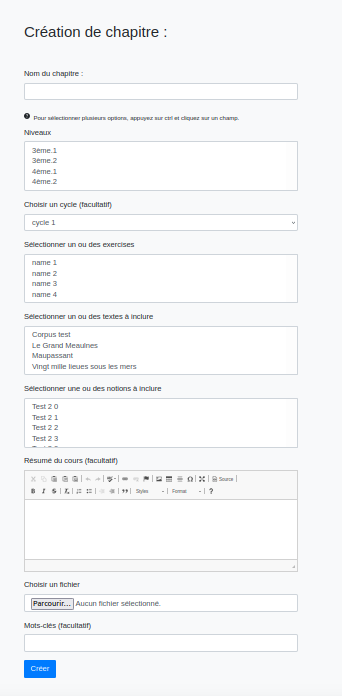
\includegraphics[scale=0.9]{crea_chap.png}
    \caption{Interface de création d'un chapitre}
    \label{fig:crea_chap}
\end{figure}

\begin{figure}
    \centering
    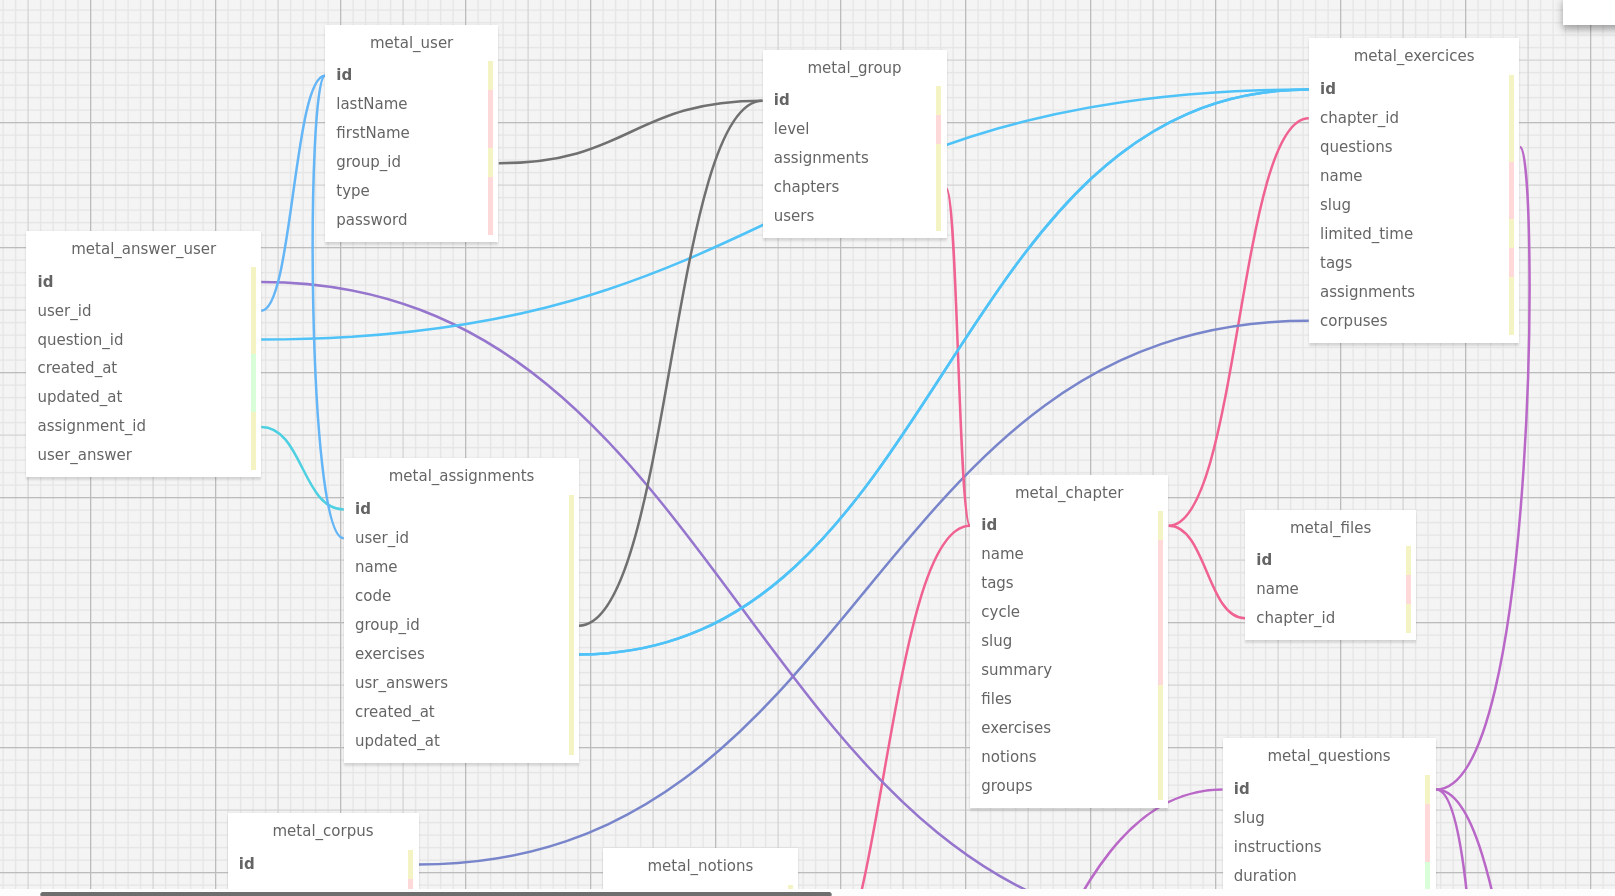
\includegraphics[scale=0.3]{uml1.png}
    \caption{Graphe UML}
    \label{fig:UML1}
\end{figure}

\begin{figure}
    \centering
    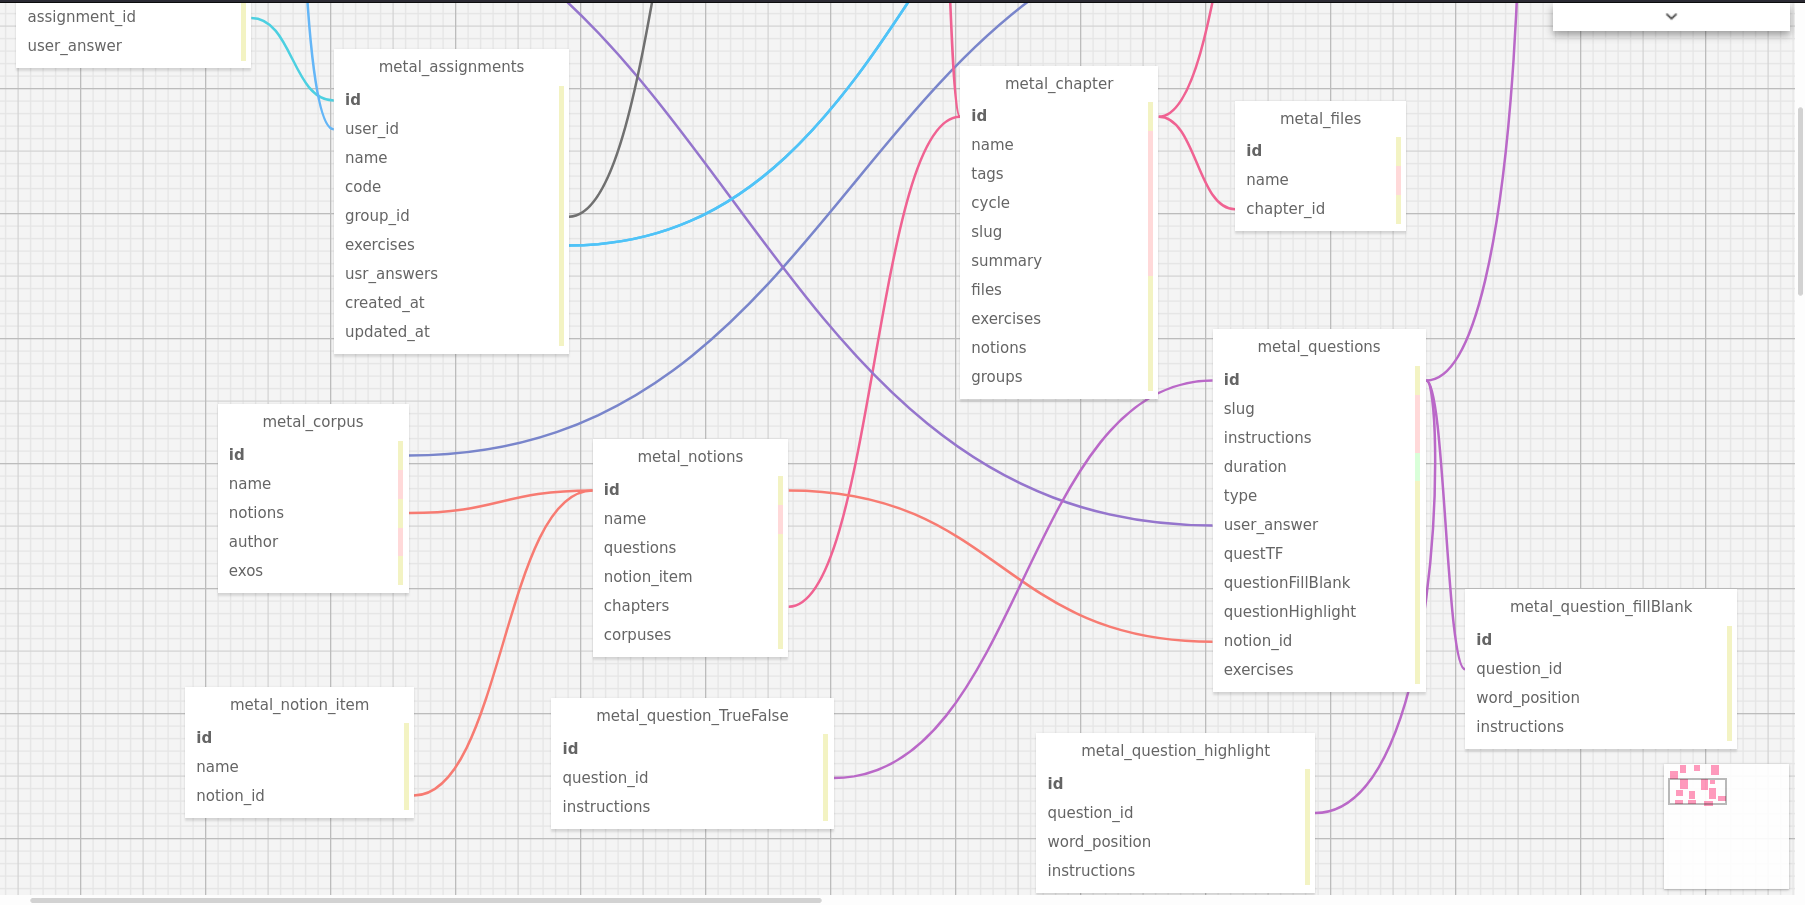
\includegraphics[scale=0.27]{uml2.png}
    \caption{Graphe UML - suite}
    \label{fig:UML2}
\end{figure}


\begin{figure}
    \centering
    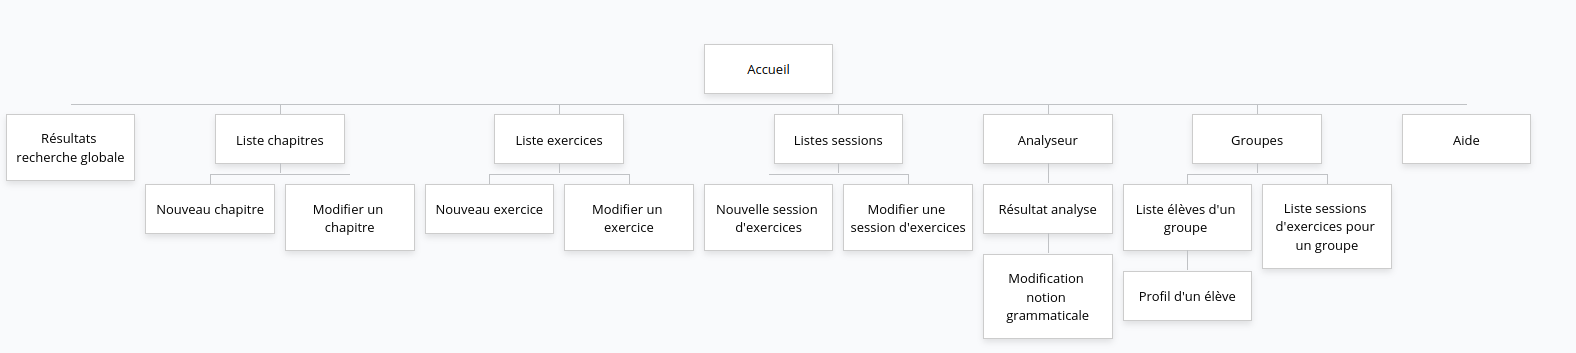
\includegraphics[scale=0.33]{arbre_pages_web.png}
    \caption{Structure des interfaces "enseignant"}
    \label{fig:arbre_pages}
\end{figure}

\begin{figure}
    \centering
    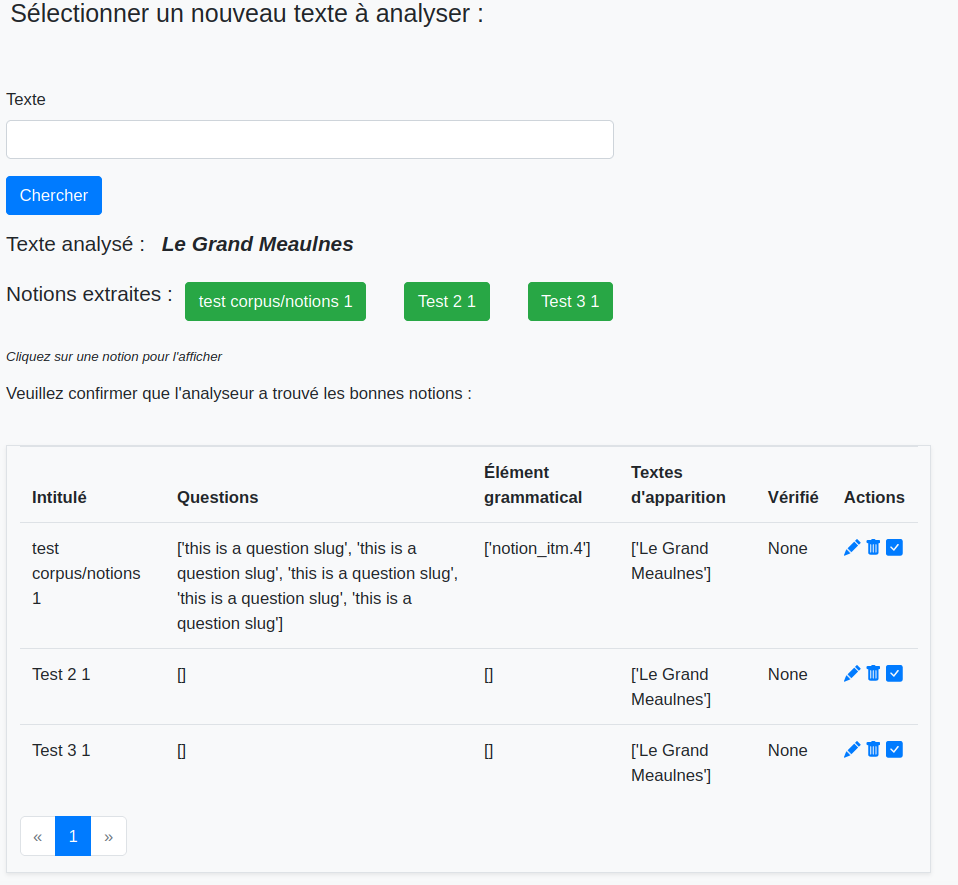
\includegraphics[scale=0.5]{analyseur_interface.png}
    \caption{Interface de l'analyseur de texte}
    \label{fig:analyseur}
\end{figure}



\clearpage
\section*{Dos du rapport}
\thispagestyle{empty}


\textbf{Etudiant (nom et prénom) :} AGUIAR Mathilde \\
\textbf{Année d’étude dans la spécialité:} INFO4 \\

\textbf{Entreprise :} LORIA \\
\textbf{Adresse complète : (géographique et postale)} \\
\textbf{Téléphone (standard) :} 03 83 59 20 00 \\

\textbf{Responsable administratif (nom et fonction) :}\\
\textbf{Téléphone:} \\
\textbf{Courriel:}\\

\textbf{Tuteur de stage (organisme d’accueil)} PARMENTIER Yannick\\
\textbf{Téléphone:} +33 3 54 95 86 58 \\
\textbf{Courriel:} yannick.parmentier@loria.fr \\

\textbf{Enseignant-référent:} MONIN Jean-François \\
\textbf{Téléphone:} \\
\textbf{Courriel:} jean-francois.monin@univ-grenoble-alpes.fr \\

\textbf{Titre : (maximum 2 à 3 lignes).} \\
Analyse et développement d’une application web dans le cadre d’un projet
d’apprentissage des langues assisté par ordinateur (Computer-Aided Language
Learning) \\
\textbf{Résumé : (minimum 15 lignes).}\\
Pour mon stage d’INFO4 j’ai eu la chance d’intégrer le LORIA et l’équipe de recherche SyNaLP. J’ai travaillé avec M.Parmentier, mon tuteur de stage, pour l’assister dans le développement d’une application d’aide à l’apprentissage des langues. Cette application a pour but de faciliter la création d’exercices ciblant des notions grammaticales particulières en proposant un analyseur de textes qui va auto-générer des questions (traitant ladite notion). 
Mon rôle était de développer la partie "enseignant" de l’application. Pour ce faire j’ai utilisé le framework léger Flask ainsi que certains plugins comme Flask WTForms, Bootstrap Flask , Flask SQLAlchemy et ses dialectes SQLite. J’ai à la fois créé les interfaces Web mais je me suis aussi occupée de redéfinir et recoder la base de données. 
Dans une seconde partie je me suis occupée de la partie traitement des langues. Pour cela j'ai dû créer un jeu de données à l'aide de textes et articles directement extraits via des techniques de Web scraping de WikiData et de la librairie libre Gutenberg. J'ai ensuite dû réaliser un modèle capable de réaliser des tâches de topic labelling pour déterminer les sujets principaux contenus dans des textes passés en entrée. 






\end{document}
